\documentclass[Report.tex]{subfiles}
\begin{document}
\emph{Principal Component Analysis}, or in short PCA, is a way to take high dimensional data and reduce it without losing much information. It is difficult to find clusters, similarities and differences in high dimensional data, but by doing PCA it becomes much easier because of the dimensions reduction. \cite{PCAtheory}

With multidimensional data plotted in a coordinate system, PCA finds the vectors which describes the most variance in the data. These are called the \emph{eigenvectors}. The eigenvector describing the most variance is the first \emph{principal component} (PC in short), the eigenvector describing the second most variance is the second PC and so on. The PCs are perpendicular. Figure \ref{fig:eigen} shows a scatter plot with the first and second PC drawn as the red and green line.
\begin{figure}
\center
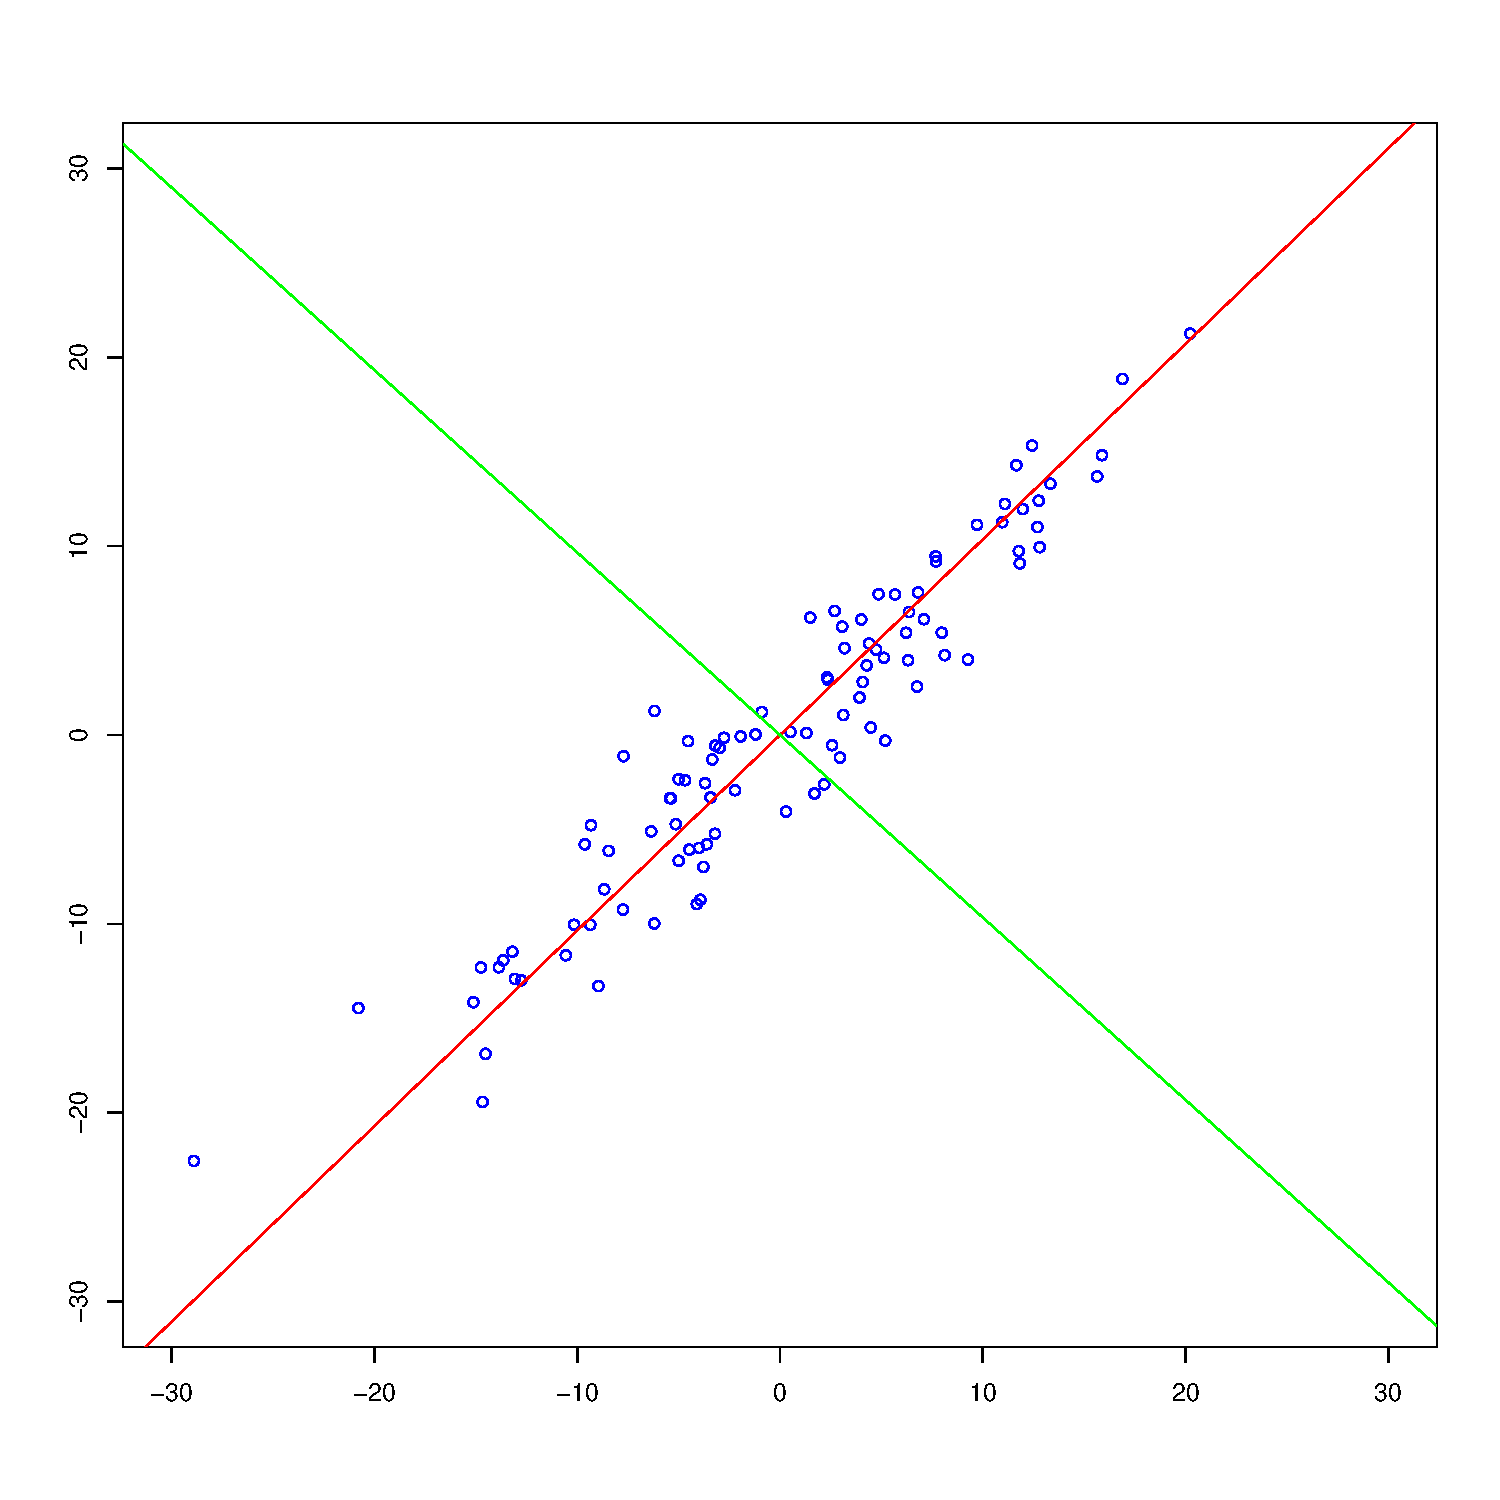
\includegraphics[width=0.5\textwidth]{Eigenvector.pdf}
\caption{Some data set plotted, red line is PC1, green is PC2}
\label{fig:eigen}
\end{figure}

To find out which variables have the most influence on a PC, we can look at the coefficients of the PC, meaning the coefficients of the eigenvector, the higher the coefficient, the higher the influence. 
When the principal components have been found, it is time to find out which to keep. This can be done by looking at a \emph{scree plot}. This is a bar chart showing the variance for each of the PCs. Typically it is interesting to look at the first two PCs. We then look at the data expressed in terms of the principal components we have chosen. If we plot the derived data as a scatter plot, with for example the first PC on the x-axis and the second PC on the y-axis, we can easily point out the clusters of the data if there are any. This way we can look at the data in fewer dimensions but without much loss of information. In section \ref{sec:PCA} we do principal components analysis on some of our own data.



\end{document}